\documentclass{article}

\PassOptionsToPackage{numbers,sort&compress}{natbib}
\usepackage[preprint]{../../neurips}
\usepackage[utf8]{inputenc}
\usepackage[T1]{fontenc}
\usepackage{hyperref}
\usepackage{url}
\usepackage{booktabs}
\usepackage{microtype}
\usepackage{xcolor}
\usepackage{graphicx}
\usepackage{subcaption}
\usepackage{multirow}
\usepackage{array}
\usepackage{adjustbox}
\usepackage{enumitem}
\usepackage{algorithm}
\usepackage{algpseudocode}
\usepackage{amsmath}
\usepackage{amssymb}
\usepackage{amsfonts}
\usepackage{amsthm}
\usepackage{mathtools}
\usepackage{bm}

\title{D-COLA: Post-hoc Domain Generalization by Mergeable Complementarity}
\author{Anonymous Authors}

\newtheorem{theorem}{Theorem}[section]
\newtheorem{proposition}[theorem]{Proposition}
\newtheorem{lemma}[theorem]{Lemma}
\newtheorem{corollary}[theorem]{Corollary}
\newtheorem{assumption}[theorem]{Assumption}
\theoremstyle{definition}
\newtheorem{definition}[theorem]{Definition}
\newtheorem{remark}[theorem]{Remark}

\newcommand{\RR}{\mathbb{R}}
\newcommand{\cA}{\mathcal{A}}
\newcommand{\cC}{\mathcal{C}}
\newcommand{\cV}{\mathcal{V}}
\newcommand{\argmin}{\operatorname*{arg\,min}}
\newcommand{\Cov}{\operatorname{Cov}}
\newcommand{\proj}{\operatorname{Proj}}
\newcommand{\TBD}{\textbf{TBD}}
\newcommand{\dcola}{\textup{\textsc{D-COLA}}}
\newcommand{\swad}{\textup{\textsc{SWAD}}}
\newcommand{\diwa}{\textup{\textsc{DiWA}}}
\newcommand{\eoa}{\textup{\textsc{EoA}}}
\newcommand{\erm}{\textup{\textsc{ERM}}}
\newcommand{\ood}{\textup{\textsc{OOD}}}
\newcommand{\one}{\mathbf{1}}
\newcommand{\simplex}{\Delta}
\newcommand{\norm}[1]{\left\lVert #1 \right\rVert}
\newcommand{\abs}[1]{\left\lvert #1 \right\rvert}
\newcommand{\inner}[2]{\left\langle #1, #2 \right\rangle}
\newcommand{\paren}[1]{\left( #1 \right)}
\newcommand{\braces}[1]{\left\{ #1 \right\}}
\newcommand{\thetaw}{\bar{\theta}(w)}

\begin{document}

\maketitle

\begin{abstract}
Current post-hoc domain generalization methods are usually justified by one proxy object: flatness of a checkpoint region, diversity of the members being averaged, or validation performance of a selected model. This paper argues that the larger object is \emph{mergeable complementarity}. A good post-hoc soup should combine checkpoints that correct different source-domain failures while still remaining averageable as one deployable model. We show that \dcola{} is a practical surrogate implementation of that principle. The rigorous theory is stated for a fixed retained checkpoint family and the convex weighting problem solved on that family; the anchor, prefilter, and barrier-screening stages used by the implementation are presented explicitly as operational heuristics motivated by the same principle, not as theorem-derived consequences. The theory is organized around one ideal objective: robust source-domain fit plus hidden-shift sensitivity plus a mergeability remainder. We prove an exact robust-domain-prior identity for the worst-domain term, an exact local hidden-shift identity on samplewise linear proxy losses, a variance and pairwise-covariance representation of the conflict matrix, and a conditional surrogate theorem showing that the practical weighting objective upper-bounds the ideal fixed-family objective under a direct mergeability certificate. We further prove convexity, projected-subgradient convergence, and a low-curvature face bound explaining why exact weights can matter less than locating the right complementary face of the simplex. Sections reporting new \dcola{} experiments remain intentionally marked \TBD{}, but we include exact published benchmark context from prior post-hoc domain generalization papers to define the target bar.
\end{abstract}

\section{Introduction}

Post-hoc domain generalization matters because it is one of the few robustness strategies that can be attached to a strong empirical-risk-minimization pipeline without retraining. A single training run produces a dense checkpoint trajectory, and one deployable model is chosen only after training has already finished. This regime is operationally attractive and already empirically validated: on DomainBed, \swad{} reported an average accuracy of \(66.9\) over PACS, VLCS, OfficeHome, TerraIncognita, and DomainNet, improving \erm{} from \(63.3\) \citep{cha2021swad}. Later weight-averaging studies pushed the frontier higher, including \diwa{}, whose strongest published linear-probe setting reports \(68.0\) average accuracy \citep{rame2022diwa}. The practical question is therefore no longer whether post-hoc averaging can help. The unresolved question is \emph{what principle the final soup should optimize}.

The dominant theoretical explanation in this niche is flatness. \swad{} states that ``finding flat minima results in a smaller domain generalization gap'' \citep{cha2021swad}. That theory is important, but it leaves two gaps. First, flatness mainly explains why averaging may be \emph{safe}; it does not fully explain why some checkpoint combinations are \emph{useful}. Second, it does not explain why post-hoc performance often depends on nonredundancy among the members being averaged, a point emphasized by later analyses of weight averaging under distribution shift. \diwa{} explicitly argues for a ``bias-variance-covariance-locality decomposition'' and states that to reduce weight averaging error under \ood{} shift, one should ``seek a good trade-off between diversity and locality'' \citep{rame2022diwa}. Flatness and diversity are therefore not competing stories. They are two visible faces of a larger object.

This paper proposes that larger object:
\begin{quote}
\textbf{Mergeable complementarity.} A post-hoc soup should combine checkpoints that make different domain-conditioned mistakes, while keeping the final average inside a regime where weight averaging still tracks predictive mixing.
\end{quote}

The method in this paper, \dcola{}, is not presented as an arbitrary combination of worst-domain validation, covariance shrinkage, and locality heuristics. Instead, it is presented as a surrogate solver for one ideal objective built from mergeable complementarity:
\begin{itemize}[leftmargin=1.3em]
    \item \textbf{Worst-domain fit}: the deployed model must not already fail on one source domain.
    \item \textbf{Complementarity}: the members of the soup should not fail on the same source slices.
    \item \textbf{Mergeability}: the weight-space average must remain a valid single-model approximation to the predictive mixture.
\end{itemize}

That single principle explains both why flat minima can generalize and why flatness is not the whole story. In a conflict-free, highly mergeable region, flatness is enough and dense uniform averaging works. Outside that limit, one needs not only mergeability but also useful disagreement. This is the regime \dcola{} targets.

The paper makes five contributions.
\begin{enumerate}[leftmargin=1.4em]
    \item We introduce \emph{mergeable complementarity} as a beyond-flatness theoretical object for post-hoc domain generalization and position \dcola{} as a surrogate implementation of that object.
    \item We derive the worst-domain term from an exact ambiguity-set identity over unknown source-domain priors and derive the covariance term from an exact local hidden-shift sensitivity identity on samplewise linear proxy losses.
    \item We show that the conflict matrix admits both variance and pairwise-covariance decompositions, making the complementarity interpretation explicit rather than rhetorical.
    \item We prove a conditional surrogate theorem for the fixed-family weighting problem, together with convexity, projected-subgradient convergence, and a low-curvature face bound explaining why exact weights may matter less than support discovery.
    \item We separate theory from implementation honestly: the rigorous contribution concerns the retained-family weighting subproblem, while worst-domain anchoring, epsilon prefiltering, and barrier screening are operational heuristics that instantiate the broader principle in the current system.
\end{enumerate}

The experimental sections remain intentionally blank for new \dcola{} results. That is deliberate. The goal of this rewrite is to make the paper theoretically coherent and publication-ready before inserting empirical tables. Exact published numbers from prior papers are included so that the benchmark bar remains concrete.

\begin{figure}[t]
    \centering
    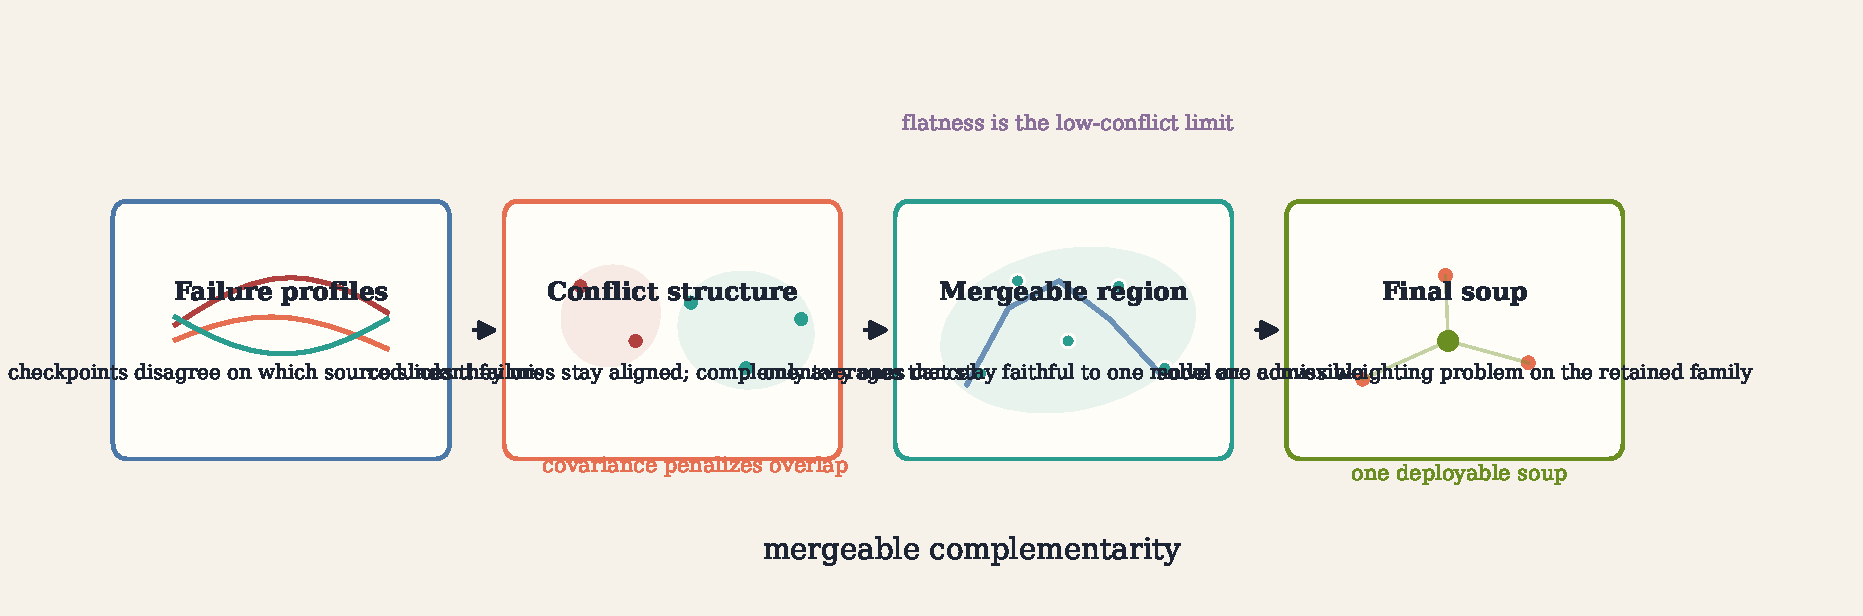
\includegraphics[width=\linewidth]{figures/dcola_overview.pdf}
    \caption{\textbf{\dcola{} at a glance.} The larger principle is mergeable complementarity: choose checkpoints that cover different domain-conditioned failures, but only inside a family whose weighted average remains a valid single model. The theorem-bearing contribution concerns the fixed-family weighting problem. The implementation then instantiates that theory with practical family-construction heuristics such as worst-domain anchoring and barrier screening.}
    \label{fig:overview}
\end{figure}

\section{Related Work}

\paragraph{Post-hoc domain generalization.}
DomainBed established that carefully tuned baselines remain difficult to beat under controlled evaluation \citep{gulrajani2021domainbed}. Within that benchmark culture, post-hoc methods are attractive because they preserve the original training pipeline. \swad{} made this niche serious by showing large gains from overfit-aware dense checkpoint averaging \citep{cha2021swad}. \eoa{} and related moving-average work further showed that averaging can stabilize selection under shift \citep{arpit2021ensemble}. These methods demonstrate that the final deployable model is often not the last checkpoint.

\paragraph{Flatness, diversity, and weight averaging.}
\swad{} argues that seeking flat minima reduces the domain generalization gap \citep{cha2021swad}. \diwa{} broadens that picture. Its abstract states that its ``main motivation is to increase the functional diversity across averaged models'' and its theory introduces a ``bias-variance-covariance-locality decomposition'' \citep{rame2022diwa}. In the DiWA source, the authors explicitly write that ``to reduce WA's error in \ood{}, we thus seek a good trade-off between diversity and locality'' \citep{rame2022diwa}. We take that sentence as the closest prior articulation of the object formalized here: the challenge is not flatness alone, but mergeable complementarity.

\paragraph{Mode connectivity and soups.}
Linear mode connectivity and model soups show that weight averaging is useful only when models occupy a common compatible basin \citep{frankle2020linear,wortsman2022soups}. This is the direct ancestor of the mergeability part of our theory. The difference is conceptual. Those works justify \emph{whether} averaging is feasible. Our theory is about \emph{which} feasible averages should be preferred for domain generalization.

\paragraph{Distribution shift and hidden subpopulations.}
The classical domain adaptation theory of \citet{ben2010theory} clarifies that source-target divergence remains uncontrollable without target information. This is why post-hoc DG can only act on the controllable source-side terms. The hidden-shift term in our analysis lives in that controllable region: it measures sensitivity to local redistributions of source support mass inside each observed source domain. The resulting theory stays source-only and post-hoc.

\section{Setup}
\label{sec:setup}

We assume \(E\) labeled source domains with held-out validation splits
\[
\cV_e = \braces{z_{e,j}}_{j=1}^{n_e},
\qquad
z_{e,j}=(x_{e,j}, y_{e,j}),
\qquad
1 \le e \le E.
\]
The post-hoc input is a dense single-run checkpoint bank
\[
\Theta_K = \braces{\theta_t}_{t=1}^{K}.
\]
For most theory statements we assume \(n_e=n\) for all \(e\), only to simplify notation; the empirical method does not require equal domain sizes.

\paragraph{Retained family.}
The rigorous theory is stated for an arbitrary retained family
\[
\cC \subseteq \braces{1,\dots,K}.
\]
Weights live on the simplex \(w\in\simplex^{|\cC|}\), and the deployed soup is
\[
\thetaw = \sum_{t\in\cC} w_t \theta_t.
\]

For checkpoint \(\theta_t\), define domainwise validation cross-entropy
\[
\widehat L_e(\theta_t)
=
\frac{1}{n}\sum_{j=1}^{n}
-\log p_{\theta_t}(y_{e,j}\mid x_{e,j}).
\]
Let
\[
\widehat L_{\max}(\theta_t) = \max_{1\le e\le E}\widehat L_e(\theta_t),
\qquad
\widehat L_{\mathrm{avg}}(\theta_t)=\frac{1}{E}\sum_{e=1}^{E}\widehat L_e(\theta_t).
\]

\paragraph{Predictive mixture quantities.}
For each retained checkpoint and validation sample, define
\[
q_{e,j,t} = p_{\theta_t}(y_{e,j}\mid x_{e,j}) \in (0,1].
\]
The predictive-mixture loss on source domain \(e\) is
\begin{equation}
\widehat L_e^{\mathrm{ens}}(w)
=
\frac{1}{n}\sum_{j=1}^{n}
-\log\paren{\sum_{t\in\cC} w_t q_{e,j,t}}.
\label{eq:ensloss}
\end{equation}
The practical \dcola{} algorithm optimizes over these cached probabilities and then outputs the actual weight soup \(\thetaw\).

\subsection{Operational family construction in the current implementation}
\label{subsec:heuristics}

The current implementation of \dcola{} does not optimize over the full checkpoint bank directly. It first builds a retained family \(\cC\) using three operational heuristics motivated by mergeable complementarity:
\begin{enumerate}[leftmargin=1.3em]
    \item choose the best singleton under worst-domain source validation loss,
    \item prefilter checkpoints within an \(\epsilon\)-window of that singleton,
    \item remove checkpoints whose interpolation barrier to the singleton exceeds a threshold \(\tau\).
\end{enumerate}
These heuristics matter operationally, but they are not the main theorem-bearing object of the paper.

The singleton anchor is
\begin{equation}
a \in \argmin_{1\le t\le K} \widehat L_{\max}(\theta_t).
\label{eq:anchor}
\end{equation}
For an interpolation grid \(\cA \subset [0,1]\), its barrier to checkpoint \(t\) is
\begin{equation}
B(t,a)
=
\max_{\alpha\in\cA}
\widehat L_{\mathrm{avg}}\paren{(1-\alpha)\theta_a + \alpha \theta_t}
-
\max\braces{\widehat L_{\mathrm{avg}}(\theta_a), \widehat L_{\mathrm{avg}}(\theta_t)}.
\label{eq:barrier}
\end{equation}
The implementation then keeps
\begin{equation}
\cC
=
\braces{
t\in\braces{1,\dots,K}:
\widehat L_{\max}(\theta_t)\le \widehat L_{\max}(\theta_a)+\epsilon,
\;
B(t,a)\le \tau
}.
\label{eq:candidates}
\end{equation}
The theory below should therefore be read as follows: once a retained family \(\cC\) has been chosen, the fixed-family weighting problem admits a clean mergeable-complementarity analysis. The anchor and barrier rules above are the concrete family-construction heuristics used by the current implementation.

\section{From One Principle to the Practical Objective}
\label{sec:principle}

\subsection{Ideal mergeable complementarity on a fixed family}

\begin{proposition}[Worst-domain fit as a robust source-domain prior]
\label{prop:worst_domain_prior}
For any retained family \(\cC\) and any \(w\in \simplex^{|\cC|}\),
\begin{equation}
\sup_{\pi\in \simplex^{E}}
\sum_{e=1}^{E} \pi_e \widehat L_e^{\mathrm{ens}}(w)
=
\max_{1\le e\le E}\widehat L_e^{\mathrm{ens}}(w).
\label{eq:worst_domain_prior}
\end{equation}
\end{proposition}

\begin{definition}[Mergeable complementarity objective]
\label{def:ideal}
Let
\begin{equation}
M(w)
:=
\max_{1\le e \le E}
\abs{
\widehat L_e(\thetaw)-\widehat L_e^{\mathrm{ens}}(w)
}
\label{eq:mergeability_remainder}
\end{equation}
be the \emph{mergeability remainder}: the gap between the actual single-model soup and the predictive mixture it is meant to approximate. Let \(C\) be the aggregate conflict matrix defined in Eq.~\eqref{eq:aggregate_conflict}. For constants \(\lambda_{\mathrm{sh}},\lambda_{\mathrm{mg}}>0\), define
\begin{equation}
\Phi(w)
:=
\max_{1\le e\le E}\widehat L_e^{\mathrm{ens}}(w)
\;+\;
\lambda_{\mathrm{sh}}\sqrt{w^\top C w}
\;+\;
\lambda_{\mathrm{mg}} M(w).
\label{eq:ideal_objective}
\end{equation}
\end{definition}

The meaning of Eq.~\eqref{eq:ideal_objective} is direct.
\begin{itemize}[leftmargin=1.3em]
    \item The first term requires the predictive mixture to fit the hardest observed source domain.
    \item The second term penalizes domain-conditioned conflict: if the chosen checkpoints make the same source-domain mistakes, the centered samplewise losses remain highly correlated and \(\sqrt{w^\top Cw}\) stays large.
    \item The third term enforces mergeability: the actual weight soup must stay close to the predictive mixture being optimized.
\end{itemize}

\subsection{Practical \dcola{} on a retained family}

\dcola{} is the practical surrogate of Eq.~\eqref{eq:ideal_objective}. Its objective is
\begin{equation}
J(w)
=
\max_{1\le e\le E}\widehat L_e^{\mathrm{ens}}(w)
\;+\;
\lambda_{\mathrm{cov}}\,w^\top C w
\;+\;
\lambda_{\mathrm{loc}}\,b^\top w
\;+\;
\lambda_{\mathrm{ent}}\sum_{t\in\cC} w_t\log w_t,
\label{eq:dcola_objective}
\end{equation}
where
\[
b_t = B(t,a),
\qquad
C = \frac{1}{E}\sum_{e=1}^{E} C_e.
\]
The first term is exact predictive-mixture fit on the hardest source domain. The second and third terms are the practical surrogates of the two theoretical penalties in Eq.~\eqref{eq:ideal_objective}. The entropy term is not part of the core theory; it is a small numerical regularizer that stabilizes optimization inside the simplex. In the implementation, \(b_t\) is instantiated by the anchor-relative interpolation barrier in Eq.~\eqref{eq:barrier}, and the optimizer returns the averaged projected-subgradient iterate rather than an exact simplex minimizer.

\begin{algorithm}[t]
\caption{\dcola{}}
\label{alg:dcola}
\begin{algorithmic}[1]
\Require Dense checkpoint bank \(\Theta_K\), source validation splits \(\{\cV_e\}_{e=1}^{E}\), thresholds \(\epsilon,\tau\), penalty coefficients \(\lambda_{\mathrm{cov}}, \lambda_{\mathrm{loc}}, \lambda_{\mathrm{ent}}\)
\State Compute \(\widehat L_e(\theta_t)\) for all \(e,t\)
\State Set anchor \(a \leftarrow \argmin_t \widehat L_{\max}(\theta_t)\)
\State Compute barriers \(B(t,a)\) by Eq.~\eqref{eq:barrier}
\State Form candidate set \(\cC\) by Eq.~\eqref{eq:candidates}
\State Cache \(q_{e,j,t}=p_{\theta_t}(y_{e,j}\mid x_{e,j})\) for all \(e,j,t\in\cC\)
\State Build domain conflict matrices \(C_e\) and aggregate \(C\)
\State Run projected subgradient descent on \(J(w)\) over \(\simplex^{|\cC|}\)
\State Return the averaged iterate \(\bar w\) and output \(\theta_{\dcola} = \sum_{t\in\cC} \bar w_t \theta_t\)
\end{algorithmic}
\end{algorithm}

\begin{figure}[t]
    \centering
    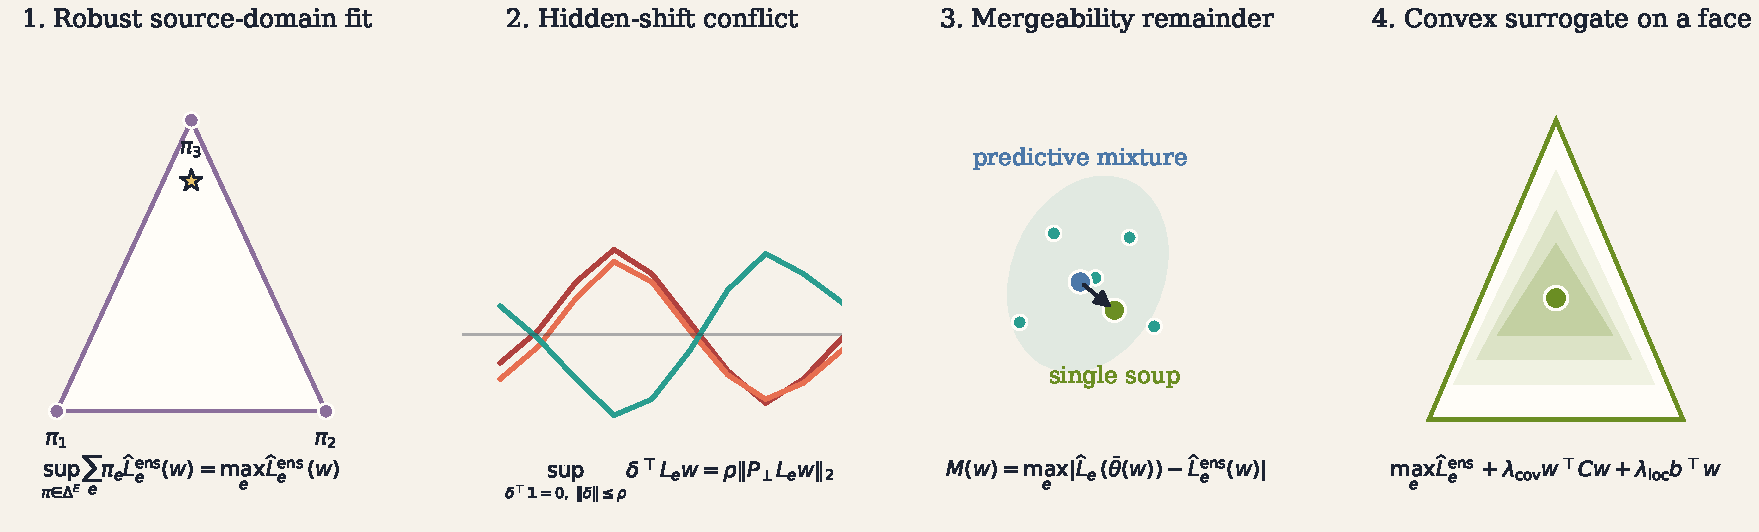
\includegraphics[width=\linewidth]{figures/dcola_surrogate_panels.pdf}
    \caption{\textbf{From ideal principle to practical surrogate.} The theory starts with a robust source-domain fit term, a hidden-shift conflict term, and a mergeability remainder. The implementation then instantiates those ideas on a retained family using a predictive-mixture surrogate, a covariance penalty, and an anchor-relative locality proxy.}
    \label{fig:steps}
\end{figure}

\section{Theory}
\label{sec:theory}

All theorem statements in this section are explicitly \emph{fixed-family}: they hold after a retained family \(\cC\) has been chosen. This is the theorem-bearing subproblem solved by the practical weighting stage. The anchor, epsilon prefilter, and barrier-screening rules in Section~\ref{subsec:heuristics} are implementation heuristics that instantiate the retained family in the current system.

\subsection{Local hidden-shift sensitivity and the conflict term}

For each domain \(e\), define the checkpoint-loss matrix
\[
L_e \in \RR^{n\times |\cC|},
\qquad
(L_e)_{j,t} = -\log q_{e,j,t}.
\]
Let
\[
u = \frac{1}{n}\one,
\qquad
P_\perp = I - \frac{1}{n}\one\one^\top.
\]
For weights \(w\in\simplex^{|\cC|}\), the samplewise linear proxy losses are
\[
\ell_e(w)=L_e w \in \RR^n.
\]
We interpret a hidden source slice inside domain \(e\) as a local reweighting of validation support mass:
\[
\alpha = u + \delta,
\qquad
\one^\top \delta = 0,
\qquad
\norm{\delta}_2 \le \rho_e.
\]

\begin{proposition}[Exact local hidden-shift identity]
\label{prop:hidden_shift}
For any domain \(e\) and any \(w\in\simplex^{|\cC|}\),
\begin{equation}
\sup_{\substack{\alpha=u+\delta\\ \one^\top\delta=0\\ \norm{\delta}_2\le \rho_e}}
\alpha^\top \ell_e(w)
=
\frac{1}{n}\one^\top L_e w
\;+\;
\rho_e \norm{P_\perp L_e w}_2.
\label{eq:exact_hidden_shift}
\end{equation}
\end{proposition}

\begin{equation}
C_e
:=
\frac{1}{n-1}L_e^\top P_\perp L_e
\in
\RR^{|\cC|\times |\cC|},
\qquad
C := \frac{1}{E}\sum_{e=1}^{E} C_e.
\label{eq:aggregate_conflict}
\end{equation}

\begin{proposition}[Variance representation of conflict]
\label{prop:variance_representation}
For every domain \(e\) and every \(w\in \simplex^{|\cC|}\),
\begin{equation}
w^\top C_e w
=
\operatorname{Var}_{j\sim \mathrm{Unif}(\{1,\dots,n\})}
\Big[
\sum_{t\in\cC} w_t (L_e)_{j,t}
\Big].
\label{eq:variance_representation}
\end{equation}
Consequently,
\begin{equation}
\norm{P_\perp L_e w}_2
=
\sqrt{(n-1)\,w^\top C_e w}.
\label{eq:centered_norm_covariance}
\end{equation}
\end{proposition}

\begin{proposition}[Pairwise covariance decomposition]
\label{prop:pairwise_covariance}
For every domain \(e\) and every \(w\in\simplex^{|\cC|}\),
\begin{equation}
w^\top C_e w
=
\sum_{t\in\cC} w_t^2 \operatorname{Var}\!\big[(L_e)_{J,t}\big]
+
2\sum_{\substack{s,t\in\cC\\ s<t}} w_s w_t \operatorname{Cov}\!\big[(L_e)_{J,s}, (L_e)_{J,t}\big],
\label{eq:pairwise_covariance}
\end{equation}
where \(J\) is uniform on \(\{1,\dots,n\}\).
\end{proposition}

\begin{corollary}[Quadratic majorizer of hidden-shift sensitivity]
\label{cor:young}
Fix \(\eta>0\). Then for every \(w\in\simplex^{|\cC|}\),
\begin{equation}
\lambda_{\mathrm{sh}}\sqrt{w^\top Cw}
\le
\frac{\lambda_{\mathrm{sh}}^2}{2\eta}
+
\frac{\eta}{2}\,w^\top Cw.
\label{eq:young_majorizer}
\end{equation}
\end{corollary}

\subsection{Mergeability remainder and the locality term}

\begin{assumption}[Second-order predictive smoothness]
\label{ass:smooth}
For every input \(x\), the probability map \(\psi_x(\theta)=p_\theta(\cdot\mid x)\) is twice continuously differentiable on \(\mathrm{conv}\braces{\theta_t:t\in\cC}\). There exists \(\beta(x)\ge 0\) such that for all \(\theta,\theta'\) in that hull,
\[
\norm{
\psi_x(\theta')-\psi_x(\theta)-\nabla\psi_x(\theta)(\theta'-\theta)
}_1
\le
\frac{\beta(x)}{2}\norm{\theta'-\theta}_2^2.
\]
\end{assumption}

\begin{assumption}[Confidence floor]
\label{ass:conf_floor}
There exists \(\eta_p>0\) such that for every domain \(e\), validation sample \(z_{e,j}\), and feasible soup weight vector \(w\),
\[
p_{\thetaw}(y_{e,j}\mid x_{e,j}) \ge \eta_p,
\qquad
\sum_{t\in\cC} w_t q_{e,j,t}\ge \eta_p.
\]
\end{assumption}

\begin{theorem}[Soup-versus-mixture translation bound]
\label{thm:soup_mix}
Under Assumptions~\ref{ass:smooth} and \ref{ass:conf_floor}, for every domain \(e\) and every \(w\in \simplex^{|\cC|}\),
\begin{equation}
\abs{
\widehat L_e(\thetaw)-\widehat L_e^{\mathrm{ens}}(w)
}
\le
\frac{\bar\beta_e}{2\eta_p}
\sum_{t\in\cC} w_t \norm{\theta_t-\thetaw}_2^2,
\label{eq:soup_mix_bound}
\end{equation}
where
\[
\bar\beta_e = \frac{1}{n}\sum_{j=1}^{n}\beta(x_{e,j}).
\]
\end{theorem}

\begin{remark}[Barrier scores as a practical mergeability proxy]
\label{rem:barrier_proxy}
Theorem~\ref{thm:soup_mix} controls the mergeability remainder \(M(w)\) by a weighted second moment of checkpoint-to-soup distances. The implementation does not evaluate that quantity directly. Instead it uses interpolation barriers \(b_t=B(t,a)\) as an operational proxy for mergeability and as a family-construction diagnostic. This is a modeling choice, not a theorem.
\end{remark}

\begin{assumption}[Direct family-level mergeability certificate]
\label{ass:direct_mergeability}
For the retained family \(\cC\), there exist nonnegative coefficients \(b_t\ge 0\) and a constant \(\Lambda>0\) such that every feasible \(w\in\simplex^{|\cC|}\) satisfies
\begin{equation}
M(w)\le \Lambda\, b^\top w.
\label{eq:direct_mergeability}
\end{equation}
\end{assumption}

\subsection{The surrogate theorem}

\begin{theorem}[D-COLA as a surrogate of fixed-family mergeable complementarity]
\label{thm:surrogate}
Assume Assumption~\ref{ass:direct_mergeability}. Fix \(\eta>0\). For every feasible \(w\in\simplex^{|\cC|}\),
\begin{equation}
\Phi(w)
\le
\max_{1\le e\le E}\widehat L_e^{\mathrm{ens}}(w)
+
\frac{\eta}{2}w^\top Cw
+
\lambda_{\mathrm{mg}}\Lambda\, b^\top w
+
\frac{\lambda_{\mathrm{sh}}^2}{2\eta}.
\label{eq:surrogate_bound}
\end{equation}
Consequently, if \(\lambda_{\mathrm{cov}}=\eta/2\) and \(\lambda_{\mathrm{loc}}=\lambda_{\mathrm{mg}}\Lambda\), then the \dcola{} objective without entropy,
\[
J_0(w)=\max_e \widehat L_e^{\mathrm{ens}}(w)+\lambda_{\mathrm{cov}}w^\top Cw+\lambda_{\mathrm{loc}}b^\top w,
\]
upper-bounds the ideal mergeable-complementarity objective up to the additive constant \(\lambda_{\mathrm{sh}}^2/(2\eta)\).
\end{theorem}

\subsection{Convexity and optimization}

\begin{assumption}[Positive cached probabilities]
\label{ass:positive_probs}
For every retained checkpoint \(t\in\cC\), domain \(e\), and validation sample \(z_{e,j}\), \(q_{e,j,t}>0\).
\end{assumption}

\begin{theorem}[Convexity of the practical objective]
\label{thm:convex}
Under Assumption~\ref{ass:positive_probs}, the \dcola{} objective \(J\) in Eq.~\eqref{eq:dcola_objective} is convex on \(\simplex^{|\cC|}\). If \(\lambda_{\mathrm{ent}}>0\), it is strictly convex on the relative interior of the simplex.
\end{theorem}

\begin{theorem}[Projected-subgradient convergence]
\label{thm:convergence}
Let \(w^\star\) minimize \(J\) over \(\simplex^{|\cC|}\). Suppose projected subgradient descent generates
\[
w^{k+1} = \proj_{\simplex^{|\cC|}}\paren{w^k-\eta g^k},
\qquad
g^k \in \partial J(w^k),
\]
and \(\norm{g^k}_2\le G\) for all \(k\). Then the Ces\`aro average \(\bar w^K=\frac{1}{K}\sum_{k=1}^{K}w^k\) satisfies
\begin{equation}
J(\bar w^K)-J(w^\star)
\le
\frac{\norm{w^1-w^\star}_2^2}{2\eta K}
+
\frac{\eta G^2}{2}.
\label{eq:convergence_rate}
\end{equation}
Choosing \(\eta=\norm{w^1-w^\star}_2/(G\sqrt{K})\) yields
\[
J(\bar w^K)-J(w^\star)\le \frac{\norm{w^1-w^\star}_2G}{\sqrt{K}}.
\]
\end{theorem}

\subsection{Low-curvature faces, near-uniform weights, and the flatness limit}

\begin{assumption}[Stable active domain on a face]
\label{ass:active_face}
Fix a support set \(S\subseteq \cC\). There exists a domain \(e^\star\) such that for every \(w\in \simplex^{|S|}\),
\[
\max_{1\le e\le E}\widehat L_e^{\mathrm{ens}}(w)=\widehat L_{e^\star}^{\mathrm{ens}}(w).
\]
\end{assumption}

\begin{theorem}[Low-curvature face bound]
\label{thm:face_bound}
Fix a support set \(S\subseteq \cC\), and let \(J_{0,S}\) denote the restriction of \(J_0\) to \(\simplex^{|S|}\). Assume Assumptions~\ref{ass:conf_floor}, \ref{ass:positive_probs}, and \ref{ass:active_face} hold on that face. Then \(J_{0,S}\) has \(L_S\)-Lipschitz gradient on the relative interior of \(\simplex^{|S|}\) with
\begin{equation}
L_S \le \frac{|S|}{\eta_p^2} + 2\lambda_{\mathrm{cov}}\norm{C_{SS}}_2.
\label{eq:face_lipschitz}
\end{equation}
If \(w_S^\star\in \mathrm{ri}(\simplex^{|S|})\) minimizes \(J_{0,S}\) and \(u_S\) is the uniform distribution on \(S\), then
\begin{equation}
J_{0,S}(u_S)-J_{0,S}(w_S^\star)
\le
\frac{L_S}{2}\norm{u_S-w_S^\star}_2^2.
\label{eq:uniform_face_gap}
\end{equation}
\end{theorem}

\begin{remark}[Flatness as the low-conflict, low-remainder regime]
\label{rem:flatness}
When a retained face of the simplex lies inside a highly mergeable valley, the family-level remainder \(M(w)\) is small, the conflict matrix \(C_{SS}\) is nearly null, and the face curvature bound in Theorem~\ref{thm:face_bound} is small. In that regime, uniform averaging on the face is near-optimal. This is the precise sense in which flatness becomes a limiting case of the larger mergeable-complementarity framework rather than a competing theory.
\end{remark}

\begin{figure}[t]
    \centering
    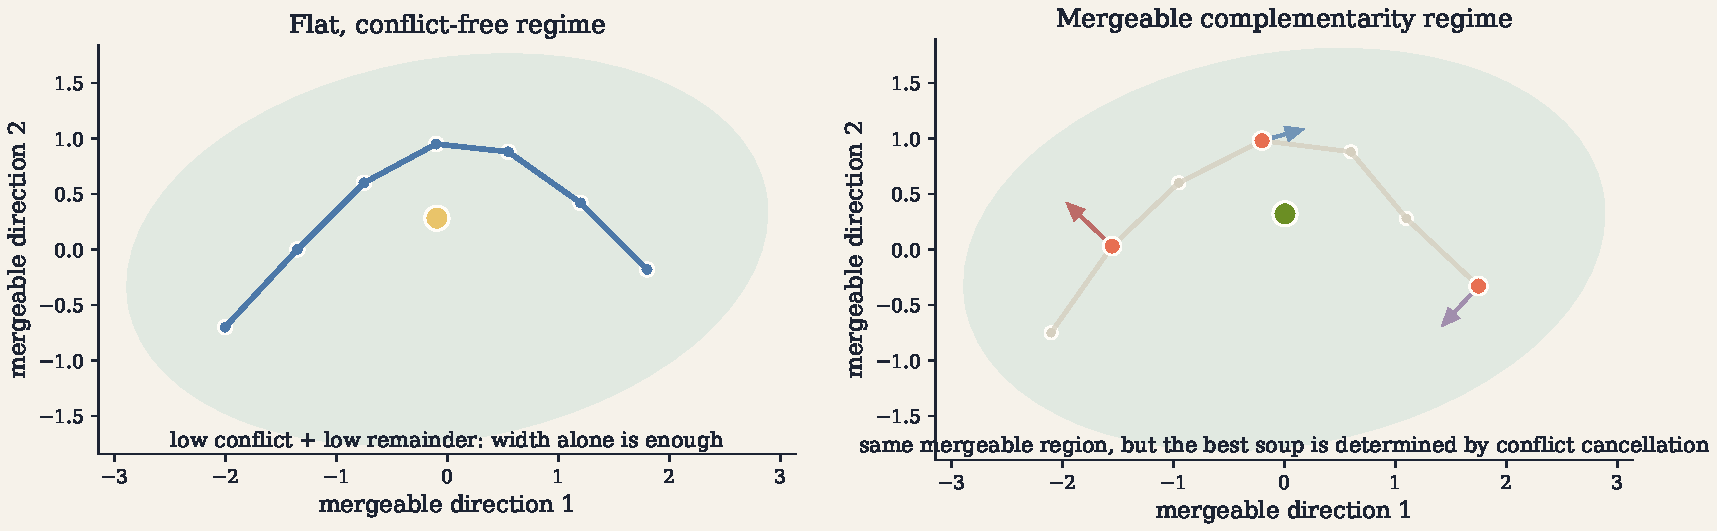
\includegraphics[width=\linewidth]{figures/dcola_2d_principle.pdf}
    \caption{\textbf{Beyond flatness in two dimensions.} Left: if the checkpoint region is flat, conflict-free, and fully mergeable, many mixtures are nearly equivalent and uniform averaging is sufficient. Right: if checkpoints remain mergeable but exhibit different domain-conditioned error profiles, the useful object is no longer flatness alone but \emph{mergeable complementarity}.}
    \label{fig:principle}
\end{figure}

\begin{figure}[t]
    \centering
    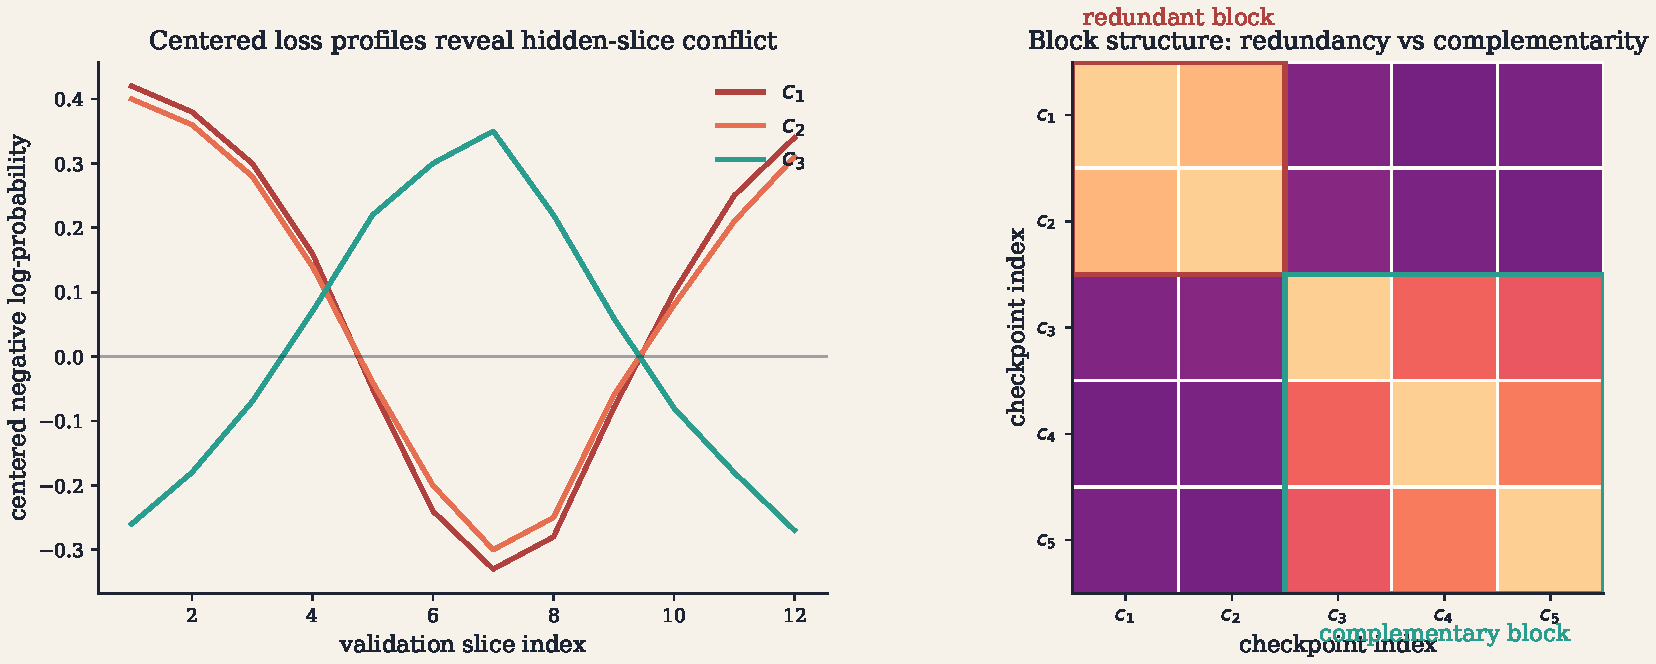
\includegraphics[width=\linewidth]{figures/dcola_hidden_shift.pdf}
    \caption{\textbf{What the covariance term is measuring.} Each checkpoint induces a samplewise validation-loss profile inside each source domain. When two checkpoints fail on the same hidden slice, their centered profiles are aligned and the conflict penalty stays large. When they cover different slices, their profiles are complementary and the weighted variance term drops.}
    \label{fig:hidden_shift}
\end{figure}

\begin{figure}[t]
    \centering
    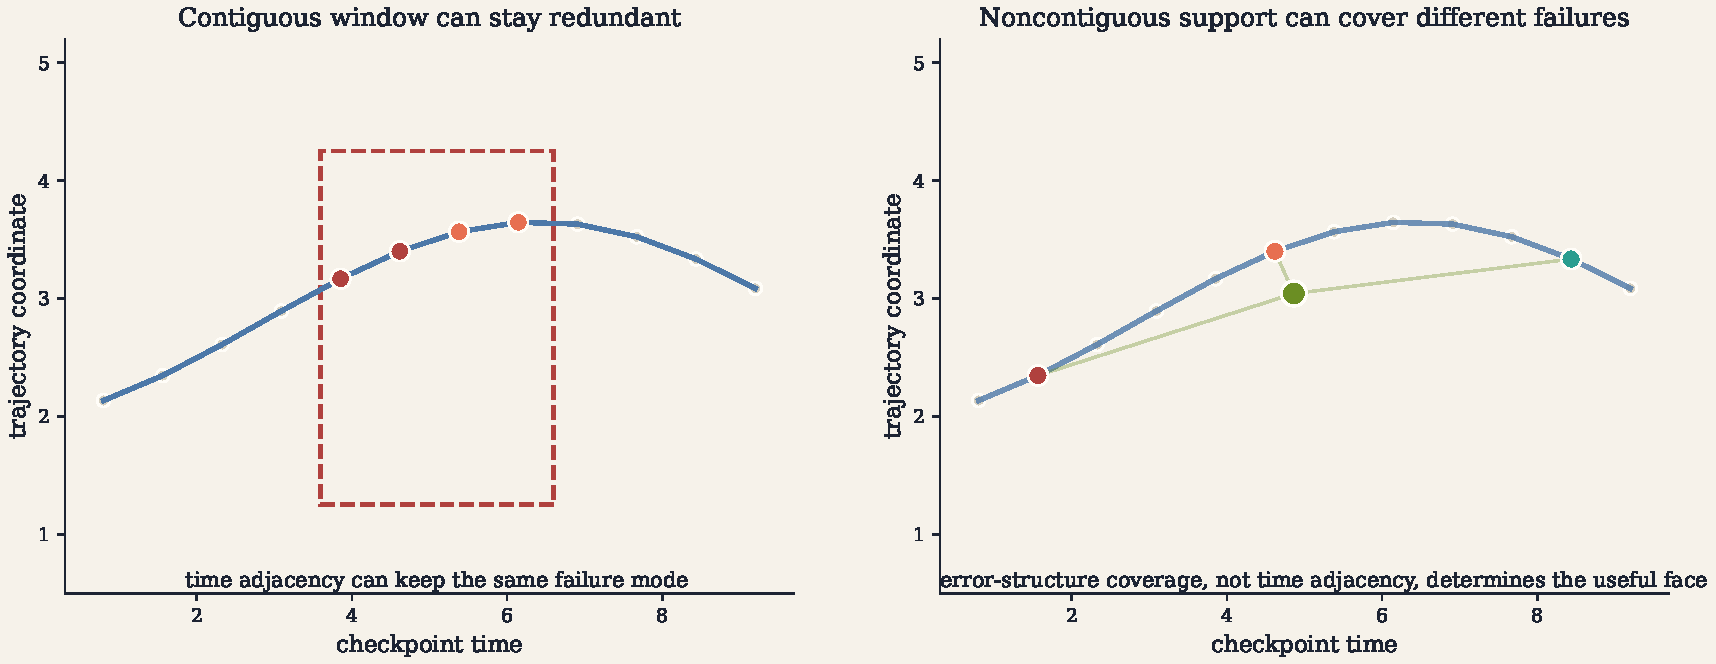
\includegraphics[width=\linewidth]{figures/dcola_noncontiguity.pdf}
    \caption{\textbf{Why noncontiguity can matter.} Contiguous windows are a time-based proxy. The mergeable-complementarity view says the actual object is error-structure coverage inside a mergeable region, so the best checkpoints need not be adjacent along training time.}
    \label{fig:noncontiguity}
\end{figure}

\begin{figure}[t]
    \centering
    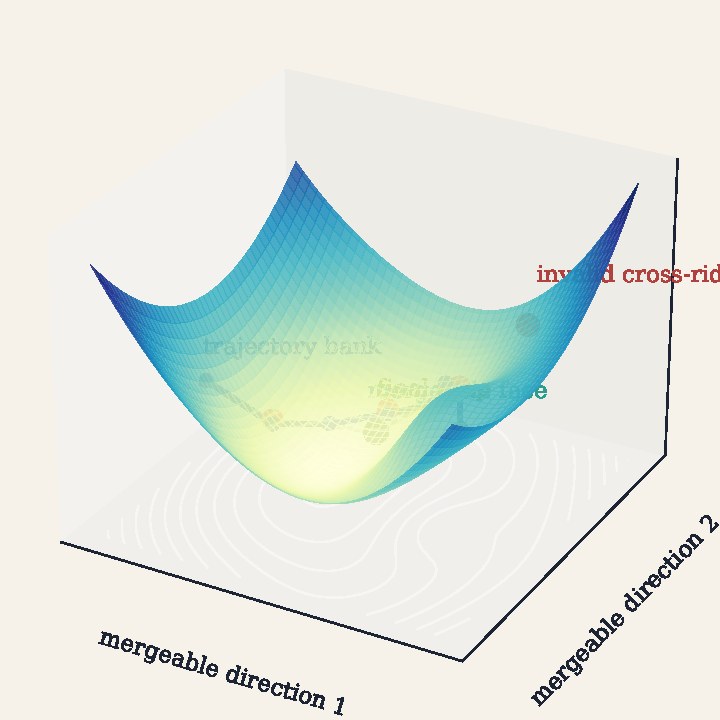
\includegraphics[width=\linewidth]{figures/dcola_3d_basin.pdf}
    \caption{\textbf{Corner-view 3D intuition.} The final object is one single soup inside a connected valley. Barrier filtering enforces mergeability, the covariance term prefers checkpoints that cancel different failure directions, and the final soup lies inside the compatible region instead of averaging blindly across the bank.}
    \label{fig:3d}
\end{figure}

\begin{figure}[t]
    \centering
    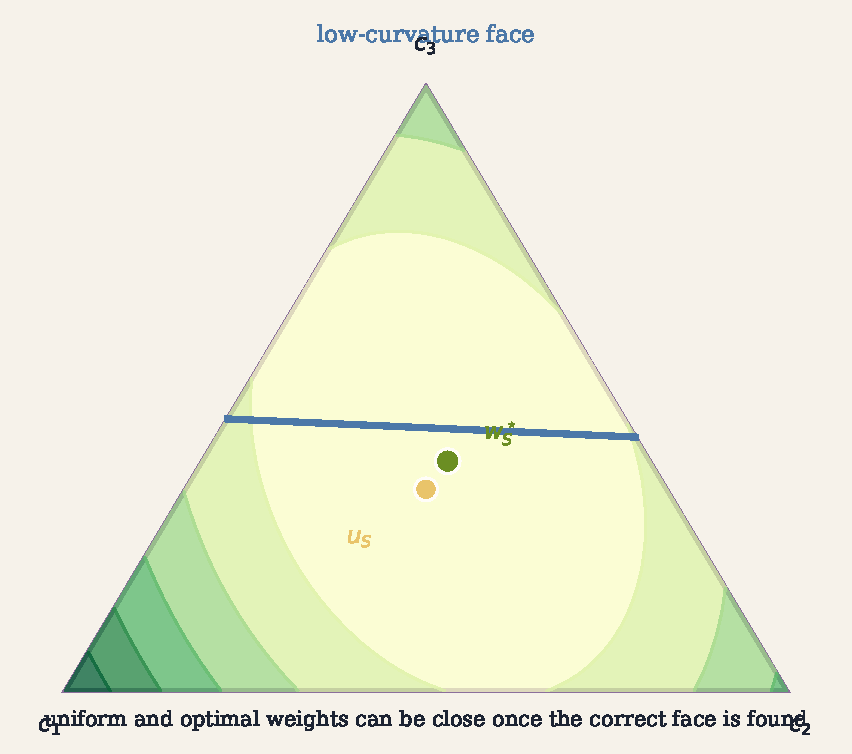
\includegraphics[width=0.86\linewidth]{figures/dcola_simplex_face.pdf}
    \caption{\textbf{Why exact weights can matter less than finding the right face.} Once the selected checkpoints lie on a low-curvature, low-conflict face of the simplex, a large region of weights can have nearly identical objective value. This is why support discovery can matter more than precise coefficient tuning.}
    \label{fig:simplex}
\end{figure}

\section{Experimental Protocol and Published Benchmark Context}
\label{sec:experiments}

The goal of this section is not to report \dcola{} numbers. Those remain intentionally blank. The goal is to define the protocol and the published benchmark context that any final empirical version of this paper must respect.

\subsection{Planned evaluation protocol}

The intended benchmark is DomainBed \citep{gulrajani2021domainbed} on PACS, VLCS, OfficeHome, TerraIncognita, and DomainNet. The primary training pipeline is standard \erm{} with dense checkpoint saving. The post-hoc selector uses only labeled source-domain validation data. The required ablations are:
\begin{itemize}[leftmargin=1.3em]
    \item remove worst-domain anchoring,
    \item remove covariance control,
    \item remove barrier filtering,
    \item remove the barrier-weight penalty while keeping the filter,
    \item replace optimized weights with uniform weights on the same retained support,
    \item compare against \swad{} and current post-hoc averaging baselines under the same backbone and data split.
\end{itemize}

\subsection{Published numbers that define the bar}

\begin{table}[t]
    \centering
    \caption{Exact published DomainBed accuracies (\%) from \swad{} and \diwa{} sources. `LP' denotes the linear-probe initialization reported by \diwa{}. These are benchmark-context numbers only; no new \dcola{} results are reported here.}
    \label{tab:published_context}
    \small
    \adjustbox{width=\textwidth}{%
    \begin{tabular}{lllcccccc}
        \toprule
        Setting & Method & Weight selection & PACS & VLCS & OfficeHome & TerraInc. & DomainNet & Avg. \\
        \midrule
        Random & \erm{} & N/A & 85.5 & 77.5 & 66.5 & 46.1 & 40.9 & 63.3 \\
        Random & \swad{} & Overfit-aware & 88.1 & 79.1 & 70.6 & 50.0 & 46.5 & 66.9 \\
        Random & MA & Uniform & 87.5 & 78.2 & 70.6 & 50.3 & 46.0 & 66.5 \\
        Random & ENS & Uniform (\(M{=}20\)) & 88.0 & 78.7 & 70.5 & 51.0 & 47.4 & 67.1 \\
        Random & \diwa{} & Restricted (\(M{\le}20\)) & 87.9 & 79.2 & 70.5 & 50.5 & 46.7 & 67.0 \\
        Random & \diwa{}\(^{\dagger}\) & Uniform (\(M{=}60\)) & 89.0 & 79.4 & 71.6 & 49.0 & 46.3 & 67.1 \\
        \midrule
        LP & \erm{} & N/A & 85.9 & 78.1 & 69.4 & 50.4 & 44.3 & 65.6 \\
        LP & MA & Uniform & 87.8 & 78.5 & 71.5 & 51.4 & 46.6 & 67.1 \\
        LP & ENS & Uniform (\(M{=}20\)) & 88.1 & 78.5 & 71.7 & 50.8 & 47.0 & 67.2 \\
        LP & \diwa{} & Restricted (\(M{\le}20\)) & 88.0 & 78.5 & 71.5 & 51.6 & 47.7 & 67.5 \\
        LP & \diwa{} & Uniform (\(M{=}20\)) & 88.7 & 78.4 & 72.1 & 51.4 & 47.4 & 67.6 \\
        LP & \diwa{}\(^{\dagger}\) & Uniform (\(M{=}60\)) & 89.0 & 78.6 & 72.8 & 51.9 & 47.7 & 68.0 \\
        \bottomrule
    \end{tabular}%
    }
\end{table}

\section{Results}
\label{sec:results}

\subsection{Main benchmark results}
\TBD{} This subsection will report the primary DomainBed table for \dcola{} under the protocol in Section~\ref{sec:experiments}, including per-dataset results and average accuracy.

\subsection{Worst-domain robustness}
\TBD{} This subsection will report whether the worst-domain source-balance objective translates into stronger OOD behavior than average-domain selectors.

\subsection{Ablations}
\TBD{} This subsection will report the anchor, covariance, barrier-filter, locality-penalty, and uniform-support ablations required to validate the mergeable-complementarity theory.

\subsection{Soup-versus-mixture diagnostics}
\TBD{} This subsection will report empirical measurements of the mergeability remainder \(M(w)\) and test whether low barrier cost really predicts a smaller soup-versus-mixture gap.

\section{Discussion}

The paper makes a deliberately narrow claim. It does not claim that \dcola{} already beats current post-hoc DG baselines; that remains an empirical question. It claims something more structural and more defensible:
\begin{quote}
The right theory object for post-hoc checkpoint soups is not flatness alone, but mergeable complementarity. \dcola{} is a practical surrogate for that object.
\end{quote}

This framing matters for three reasons.
\begin{itemize}[leftmargin=1.3em]
    \item It explains why barrier filtering and locality can matter in this implementation without pretending that flatness alone selects the right soup.
    \item It explains why covariance reduction matters without drifting into pure diversity rhetoric that ignores averageability.
    \item It clarifies the position of prior flatness-based methods: they are not wrong; they are the limiting regime where conflict and mergeability remainder are already negligible.
\end{itemize}

Three limitations are immediate.
\begin{itemize}[leftmargin=1.3em]
    \item The rigorous contribution lives on a retained family \(\cC\). The anchor, epsilon prefilter, and barrier-screening stages of the implementation are motivated by the same principle, but they are not theorem-derived consequences of it.
    \item The conflict derivation uses local source-supported hidden shifts inside the validation domains. This is principled and source-only, but it is still an approximation to unseen target structure and is exact only for the linear proxy \(L_e w\), not for the deployed soup loss.
    \item The direct mergeability certificate \(M(w)\le \Lambda b^\top w\) is a conditional modeling assumption. Interpolation barriers are one plausible empirical proxy for that certificate, but not a universal one.
\end{itemize}

\section{Conclusion}

\dcola{} is a post-hoc DG method, but the point of this rewrite is not merely to describe an algorithm. The point is to show that the algorithm can be understood as one coherent implementation of a larger theory. That theory is mergeable complementarity: combine checkpoints that cover different domain-conditioned failures, but only inside a family where one actual weight soup remains faithful to the predictive mixture. In this view, flatness is not discarded. It is explained as the low-conflict, low-remainder limit of the larger object. The honest scope is now explicit: the rigorous results concern the fixed-family weighting problem, and the current family-construction stages are operational heuristics motivated by the same theory. Whether the method ultimately clears the empirical bar remains a question for the \TBD{} sections. The theory, however, is now explicit, centralized, and falsifiable.

\bibliographystyle{plainnat}
\bibliography{d_cola_refs}

\appendix

\section{Proofs}

\subsection{Proof of Proposition~\ref{prop:worst_domain_prior}}

\begin{proof}
For any \(\pi\in \simplex^{E}\),
\[
\sum_{e=1}^{E}\pi_e \widehat L_e^{\mathrm{ens}}(w)
\le
\max_{1\le e\le E}\widehat L_e^{\mathrm{ens}}(w)
\cdot \sum_{e=1}^{E}\pi_e
=
\max_{1\le e\le E}\widehat L_e^{\mathrm{ens}}(w).
\]
Equality is attained by taking \(\pi\) to be any vertex of \(\simplex^{E}\) supported on an index \(e^\star\in\arg\max_e \widehat L_e^{\mathrm{ens}}(w)\).
\end{proof}

\subsection{Proof of Proposition~\ref{prop:hidden_shift}}

\begin{proof}
Fix a domain \(e\) and weights \(w\in\simplex^{|\cC|}\). For any admissible perturbation \(\delta\) with \(\one^\top\delta=0\),
\[
\delta^\top \ell_e(w)
=
\delta^\top P_\perp \ell_e(w),
\]
because \(P_\perp\) is the orthogonal projector onto the subspace orthogonal to \(\one\). Therefore
\[
\sup_{\substack{\one^\top\delta=0\\ \norm{\delta}_2\le \rho_e}}
\delta^\top \ell_e(w)
=
\sup_{\norm{\delta}_2\le \rho_e}\delta^\top P_\perp \ell_e(w).
\]
By Cauchy--Schwarz,
\[
\delta^\top P_\perp \ell_e(w)
\le
\norm{\delta}_2 \norm{P_\perp \ell_e(w)}_2
\le
\rho_e \norm{P_\perp \ell_e(w)}_2.
\]
Equality is attained when \(P_\perp \ell_e(w)\neq 0\) by choosing
\[
\delta^\star
=
\rho_e \frac{P_\perp \ell_e(w)}{\norm{P_\perp \ell_e(w)}_2}.
\]
If \(P_\perp \ell_e(w)=0\), both sides are zero. Since \(\alpha=u+\delta\),
\[
\sup_{\alpha}\alpha^\top \ell_e(w)
=
\frac{1}{n}\one^\top \ell_e(w) + \rho_e \norm{P_\perp \ell_e(w)}_2.
\]
Substituting \(\ell_e(w)=L_e w\) yields Eq.~\eqref{eq:exact_hidden_shift}.
\end{proof}

\subsection{Proof of Proposition~\ref{prop:variance_representation}}

\begin{proof}
Let \(\widetilde L_e = P_\perp L_e\). Then
\[
C_e = \frac{1}{n-1}\widetilde L_e^\top \widetilde L_e.
\]
For a uniformly sampled validation index \(J\in\braces{1,\dots,n}\),
\[
\operatorname{Var}\Big[\sum_t w_t (L_e)_{J,t}\Big]
=
\frac{1}{n-1}\sum_{j=1}^{n}\Big(\sum_t w_t (\widetilde L_e)_{j,t}\Big)^2
=
\frac{1}{n-1}\norm{\widetilde L_e w}_2^2
=
w^\top C_e w.
\]
This proves Eq.~\eqref{eq:variance_representation}. Since variances are nonnegative, \(C_e\succeq 0\); averaging preserves positive semidefiniteness. Finally,
\[
\norm{P_\perp L_e w}_2^2
=
\norm{\widetilde L_e w}_2^2
=
(n-1)w^\top C_e w.
\]
\end{proof}

\subsection{Proof of Proposition~\ref{prop:pairwise_covariance}}

\begin{proof}
By Proposition~\ref{prop:variance_representation},
\[
w^\top C_e w
=
\operatorname{Var}\!\Big[\sum_{t\in\cC} w_t (L_e)_{J,t}\Big].
\]
Expanding the variance of a weighted sum gives
\[
\operatorname{Var}\!\Big[\sum_{t\in\cC} w_t (L_e)_{J,t}\Big]
=
\sum_{s,t\in\cC} w_s w_t \operatorname{Cov}\!\big[(L_e)_{J,s},(L_e)_{J,t}\big].
\]
Splitting diagonal and off-diagonal terms yields Eq.~\eqref{eq:pairwise_covariance}.
\end{proof}

\subsection{Proof of Corollary~\ref{cor:young}}

\begin{proof}
Set \(x=\sqrt{w^\top Cw}\). By Young's inequality \(ab\le a^2/(2\eta)+\eta b^2/2\),
\[
\lambda_{\mathrm{sh}}x
\le
\frac{\lambda_{\mathrm{sh}}^2}{2\eta}
+
\frac{\eta x^2}{2}
=
\frac{\lambda_{\mathrm{sh}}^2}{2\eta}
+
\frac{\eta}{2}w^\top Cw.
\]
\end{proof}

\subsection{Proof of Theorem~\ref{thm:soup_mix}}

\begin{proof}
Fix domain \(e\), validation sample \((x,y)\), and weights \(w\). Let
\[
\bar\psi_w(x)=\sum_{t\in\cC} w_t p_{\theta_t}(\cdot\mid x).
\]
By Assumption~\ref{ass:smooth}, for each \(t\in\cC\),
\[
p_{\theta_t}(\cdot\mid x)
=
p_{\thetaw}(\cdot\mid x)
+
\nabla p_{\thetaw}(\cdot\mid x)(\theta_t-\thetaw)
+
r_t(x),
\]
with \(\norm{r_t(x)}_1 \le \frac{\beta(x)}{2}\norm{\theta_t-\thetaw}_2^2\). Summing against \(w_t\) cancels the first-order term because \(\sum_t w_t(\theta_t-\thetaw)=0\). Hence
\[
\norm{\bar\psi_w(x)-p_{\thetaw}(\cdot\mid x)}_1
\le
\sum_t w_t \norm{r_t(x)}_1
\le
\frac{\beta(x)}{2}\sum_t w_t \norm{\theta_t-\thetaw}_2^2.
\]
On the region where the true-class probability is at least \(\eta_p\), the map \(v\mapsto -\log v_y\) is \(1/\eta_p\)-Lipschitz in \(\ell_1\). Assumption~\ref{ass:conf_floor} therefore gives
\[
\abs{
-\log p_{\thetaw}(y\mid x)
-
\Big(-\log \sum_t w_t q_{e,j,t}\Big)
}
\le
\frac{\beta(x)}{2\eta_p}\sum_t w_t \norm{\theta_t-\thetaw}_2^2.
\]
Averaging over domain-\(e\) validation samples proves Eq.~\eqref{eq:soup_mix_bound}.
\end{proof}

\subsection{Proof of Theorem~\ref{thm:surrogate}}

\begin{proof}
Starting from Eq.~\eqref{eq:ideal_objective}, apply Corollary~\ref{cor:young} to \(\lambda_{\mathrm{sh}}\sqrt{w^\top Cw}\) and Assumption~\ref{ass:direct_mergeability} to \(M(w)\). The claimed inequality follows by substitution.
\end{proof}

\subsection{Proof of Theorem~\ref{thm:convex}}

\begin{proof}
For each sample, \(w\mapsto \sum_t w_t q_{e,j,t}\) is affine and strictly positive. Since \(u\mapsto -\log u\) is convex, each samplewise predictive-mixture loss is convex in \(w\), and so is each domain mean. The maximum over domains is convex. Proposition~\ref{prop:variance_representation} gives \(C\succeq 0\), so \(w^\top Cw\) is convex. The locality term is linear. The entropy term \(\sum_t w_t\log w_t\) is convex on the simplex and strictly convex on its relative interior. Summing the terms yields the claim.
\end{proof}

\subsection{Proof of Theorem~\ref{thm:convergence}}

\begin{proof}
Projection onto a closed convex set is nonexpansive:
\[
\norm{w^{k+1}-w^\star}_2^2
\le
\norm{w^k-\eta g^k-w^\star}_2^2.
\]
Expanding the right-hand side and rearranging,
\[
\inner{g^k}{w^k-w^\star}
\le
\frac{\norm{w^k-w^\star}_2^2-\norm{w^{k+1}-w^\star}_2^2}{2\eta}
+
\frac{\eta}{2}\norm{g^k}_2^2.
\]
The subgradient inequality gives
\[
J(w^k)-J(w^\star)\le \inner{g^k}{w^k-w^\star}.
\]
Summing over \(k=1,\dots,K\) and using \(\norm{g^k}_2\le G\) yields
\[
\sum_{k=1}^{K}\big(J(w^k)-J(w^\star)\big)
\le
\frac{\norm{w^1-w^\star}_2^2}{2\eta}
+
\frac{\eta K G^2}{2}.
\]
Convexity of \(J\) implies
\[
J(\bar w^K)\le \frac{1}{K}\sum_{k=1}^{K}J(w^k),
\qquad
\bar w^K=\frac{1}{K}\sum_{k=1}^{K}w^k.
\]
Dividing by \(K\) proves Eq.~\eqref{eq:convergence_rate}. The \(O(K^{-1/2})\) rate follows from the stated stepsize choice.
\end{proof}

\subsection{Proof of Theorem~\ref{thm:face_bound}}

\begin{proof}
Under Assumption~\ref{ass:active_face}, the restriction of \(J_{0,S}\) to the face is
\[
J_{0,S}(w)=\widehat L_{e^\star}^{\mathrm{ens}}(w)+\lambda_{\mathrm{cov}}w^\top C_{SS}w+\lambda_{\mathrm{loc}}b_S^\top w.
\]
For a fixed sample \(j\), let \(q_j\in\RR^{|S|}\) collect the true-class probabilities \(q_{e^\star,j,t}\) over \(t\in S\). Then
\[
\nabla^2\!\big(-\log(q_j^\top w)\big)=\frac{q_j q_j^\top}{(q_j^\top w)^2}.
\]
Assumption~\ref{ass:conf_floor} gives \(q_j^\top w\ge \eta_p\), so
\[
\norm{\nabla^2(-\log(q_j^\top w))}_2 \le \frac{\norm{q_j}_2^2}{\eta_p^2}\le \frac{|S|}{\eta_p^2},
\]
since each coordinate of \(q_j\) lies in \((0,1]\). Averaging over samples preserves this bound for \(\widehat L_{e^\star}^{\mathrm{ens}}\). The Hessian of \(\lambda_{\mathrm{cov}}w^\top C_{SS}w\) is \(2\lambda_{\mathrm{cov}}C_{SS}\), and the locality term is affine. Therefore the gradient of \(J_{0,S}\) is \(L_S\)-Lipschitz with \(L_S\) bounded as in Eq.~\eqref{eq:face_lipschitz}.

Now let \(w_S^\star\in \mathrm{ri}(\simplex^{|S|})\) minimize \(J_{0,S}\). By the KKT conditions on the simplex face, there exists \(\nu\in\RR\) such that
\[
\nabla J_{0,S}(w_S^\star)=\nu \one
\]
on the active coordinates. Since both \(u_S\) and \(w_S^\star\) lie on the same face,
\[
\inner{\nabla J_{0,S}(w_S^\star)}{u_S-w_S^\star}
=
\nu\,\one^\top(u_S-w_S^\star)=0.
\]
The descent lemma for \(L_S\)-smooth functions therefore gives
\[
\begin{aligned}
J_{0,S}(u_S)
&\le
J_{0,S}(w_S^\star)
+
\inner{\nabla J_{0,S}(w_S^\star)}{u_S-w_S^\star}
+
\frac{L_S}{2}\norm{u_S-w_S^\star}_2^2 \\
&=
J_{0,S}(w_S^\star)
+
\frac{L_S}{2}\norm{u_S-w_S^\star}_2^2.
\end{aligned}
\]
This is Eq.~\eqref{eq:uniform_face_gap}.
\end{proof}

\end{document}
